\documentclass{scrartcl}
\usepackage[utf8]{inputenc}
\usepackage[english]{babel} % Trennung nach der neuen deutschen Rechtschreibung
\usepackage[utf8]{inputenc}
\usepackage[T1]{fontenc}
\usepackage{lmodern}
\usepackage{subcaption}
\usepackage{chemformula}
\usepackage{placeins}
\usepackage{multirow}
\usepackage{enumitem}
\usepackage{amssymb}
\usepackage{amsmath} % Erweiterte Mathematik-Umgebung
\usepackage{amsfonts} % zusätzliche Mathematik-Schrifttypen (v.a. \mathbb für Mengen)
\usepackage{ulem}
\usepackage{amsthm}
\usepackage{graphics}%soll beim Graphiken einfügen hilfreich sein
\usepackage{graphicx}
\usepackage{wrapfig}%lässt Textumflossene Bildeinbindung zu
\usepackage{epstopdf}%soll eps in pdf umwandeln
\usepackage{placeins}
\usepackage{amsthm}
\usepackage{subcaption}
\usepackage{wrapfig}
\usepackage{float}
\usepackage{hyperref}
\usepackage{ragged2e}

\usepackage[a4paper, portrait, margin=2.5cm]{geometry}

\setlength\parindent{0pt}

\begin{document}

\begin{titlepage}
    \begin{center}
        \vspace*{1cm}
        \Huge
        \textbf{Heat engines}
        
        \vspace{0.5cm}
        \LARGE
        Advanced Lab Course
        
        \vspace{1.5cm}
        \textbf{Louis-Hendrik Barboutie (020157041C) and Florence Schmerber (0201845640)}
        
        \vspace{1cm}
        Supervisor: Evelyn Pratami SINAGA
        \vfill
        

        \includegraphics[width=0.4\textwidth]{logo_uni.jpg}
        
        \Large
        31st March 2022
    \end{center}
\end{titlepage}

\clearpage

\tableofcontents

\listoffigures
	
\clearpage

\section{Introduction}
Thermodynamic machines are not as uncommon as it may seem. One of the most widely used is the so-called heat pump. It is a device which uses the thermodynamic properties of a refrigerant to extract heat from the atmosphere and heat a closed cycle. It works by running a liquid in a loop, which is in some point in contact with the atmosphere. It absorbs the heat from it and then gets compressed, which raises its temperature, which can be used to heat water or for other domestic uses. It is then decompressed and run through the loop again. We will see more in detail how such machines work in the following report.

In this lab course we will be studying thermodynamic principles through analysing a so called heat engine. Its purpose is to convert heat into mechanical energy and is widely used in engineering, for example the same process is used for Diesel motors.
Today we will be analyzing two different cycles: the three-cycle process as well as the reversed Otto cycle.(The latter describes a four stroke gasoline engine.)

\section{Theoretical background}

The behaviour of ideal gases can be described by the ideal gas law $pV = nRT$, where p is the pressure of the gas, V the volume it occupies and T its temperature. The amount of moles of the gas is given by n and $R = N_a *k_B$ is the ideal gas constant. Since the properties of a gas are tied to each other, they change if one parameter varies. Our experiment gives us the ability to vary the volume of a gas (also how fast this variation takes place). We can then do specific cycles of these parameters, called 3-segment cycle and reversed Otto cycle. They consist of a series of processes, where the gas goes through variations of pressure, volume, and temperature, and back to the starting conditions. This makes it a "thermodynamic machine" whose efficiency we can measure, ie. how much work $W_{out}$ the machine does against how much heat input $Q_{in}$ the machine needs to function. \begin{equation} \eta = \frac{W_{out}}{Q_{in}} \end{equation} The processes we use are: \begin{enumerate} \item adiabatic: a process with no heat loss of the system to the exterior. \item isochoric: a process where the volume of the gas is held constant. \item isothermal: a process where the temperature of the gas is held constant. \end{enumerate} 

The 3-segment cycle (see figure \ref{fig:3seg pic}) consists of an adiabatic compression, followed by an isochoric cooling and finalized by an isothermal expansion. 

The reversed Otto cycle (see figure \ref{fig:Otto pic}) is a four segment cycle consisting of an adiabatic compression followed by an isochoric cooling, and then an adiabatic expansion followed by an isochoric heating.

\begin{figure}[!ht]
     \centering
     \begin{subfigure}[b]{0.45\textwidth}
         \centering
         \includegraphics[width=\textwidth]{3seg_pic.png}
         \caption{Three-segment cycle}
         \label{fig:3seg pic}
     \end{subfigure}
     \hfill
     \begin{subfigure}[b]{0.45\textwidth}
         \centering
         \includegraphics[width=\textwidth]{Otto_pic.png}
         \caption{Reversed Otto cycle}
         \label{fig:Otto pic}
     \end{subfigure}
\end{figure}
\FloatBarrier

The formulas to determine the work W, the change in internal energy $\Delta U$ and the change in entropy $\Delta S$ during the different processes can be seen in table~(\ref{tab:formulas}).\cite{adiabaticIndex}\cite{isochoricProcess}\cite{isothermalProcess}
\begin{table}[!ht]
    \centering
    \begin{tabular}{c|ccc}
         & Adiabatic & Isochoric & Isothermal  \\ \hline
        W & $\int_{V_1}^{V_2} p dV$ & 0 & $-nRTln(\frac{V_2}{V_1})$ \\ \hline
        $\Delta U$ & $n c_V \Delta T$ & $n c_V \Delta T$ & 0 \\ \hline
        $\Delta S$ & 0 & $nc_Vln(\frac{T_2}{T_1})$ & $nRln(\frac{V_2}{V_1})$
    \end{tabular}
    \caption{Formulas for work, internal energy and entropy}
    \label{tab:formulas}
\end{table}

\section{Experimental setup \& procedure}
The setup (see figure \ref{fig:setup}) is composed of a tube, that will be filled with gas and a lever that can compress the gas inside the tube when you push it down and thus increasing the pressure. We have at our disposal four gases: air, carbon dioxide, helium and argon. By pulling the lever down or up we can create the three-segment cycle (like how it's shown on figure \ref{fig:3seg pic}) and the reversed Otto cycle (figure \ref{fig:Otto pic}).\\
\begin{wrapfigure}{r}{6cm}
    \includegraphics[width=0.4\textwidth]{Setup/md_gJyTdLSiaUR8.png}
    \caption{adiabatic gas-law apparatus}
    \label{fig:setup}
\end{wrapfigure}
To create the three-segment cycle, we first have to pull down the lever hard and fast, in order to have an adiabatic process. Then we have to wait for the temperature to cool down. As we are not changing the pressure or volume in this segment, this will be the isochoric process. And finally we lift the lever slowly, holding the temperature constant, releasing the pressure and thus increasing the volume. This is the isothermal process.\\
We follow the same procedure as before to make the reversed Otto cycle but with some few changes. The first two steps stay the same. Once the gas is cooled down and holds a constant temperature, we pull the lever up for a short amount of time, then we lift the lever in one go, creating the constant volume heating process.

\section{Results}

\textit{Note}: Since there are very many values to determine, we will perform all calculations and computation for air only.

\subsection{Three-segement cycle}

\subsubsection{Air}
The recorded PV diagram for air is the following:
\begin{figure}[h]
    \centering
    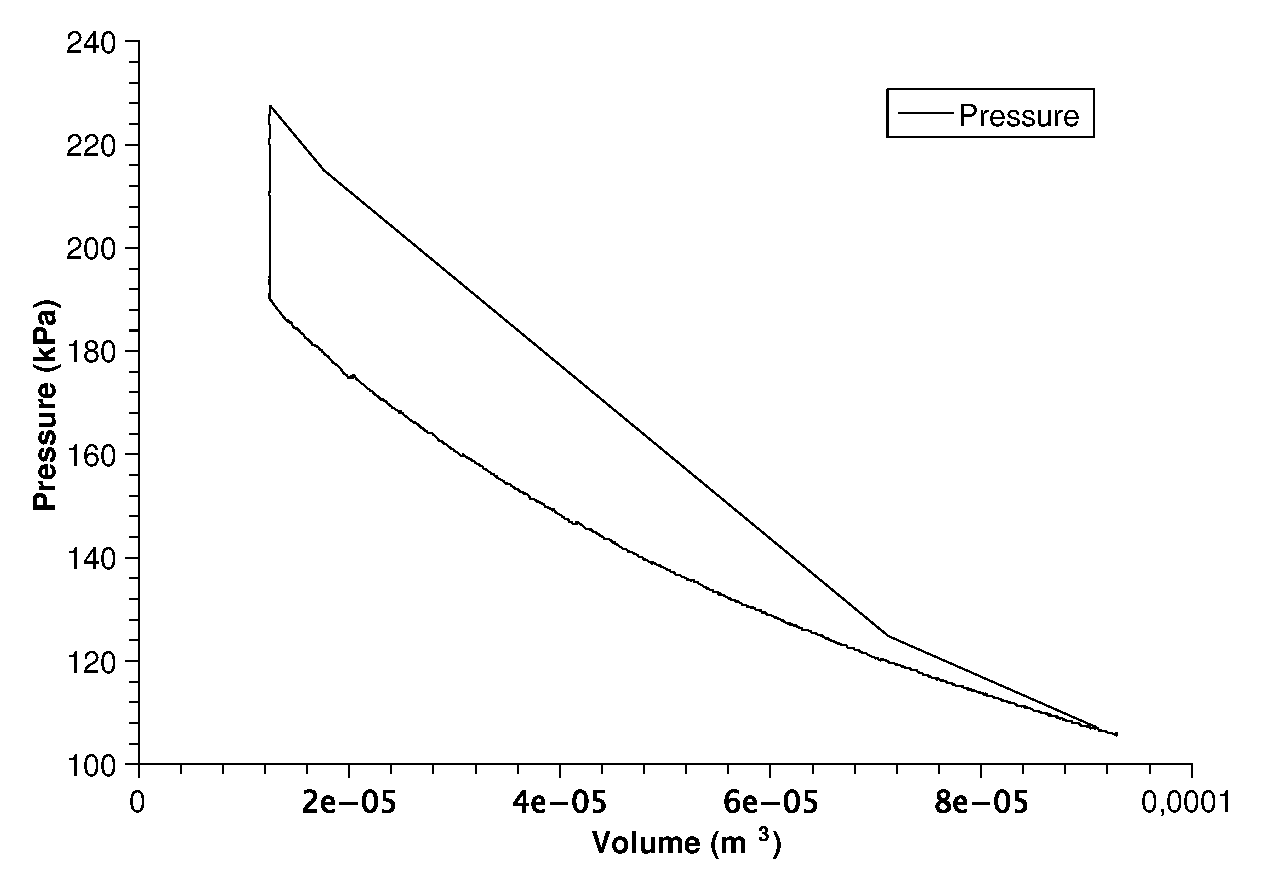
\includegraphics[width=0.5\textwidth]{3seg/PV_air_3.eps}
    \caption{P(V) diagram for the three segment cycle of air}
    \label{fig:3seg_air}
\end{figure}
\FloatBarrier

With this graph and using the ideal gas law $PV = nRT$, we can determine the amount of mole $n_{air}$ and mass inside the apparatus.
We get:
\[\ n_{air} = 2,83 \cdot 10^{-3} mol \]\
Using $m_{air} = M_{air}\cdot n_{air}$, knowing that the average molar mass of air is $M_{air} = 28.97 g/mol$ we get:
\[\ m_{air} = 8,2 \cdot 10^{-5} kg \]\ 
\vspace{0.5cm}

Next, using figure \ref{fig:3seg_air} we can determine the three limiting points (like on figure \ref{fig:3seg pic})
\begin{table}[!ht]
    \centering
    \begin{tabular}{c|c|c|c}
        point & V ($m^3$) & p (kPa) & T (K)  \\
        \hline
        1 & $9,09 \cdot 10^{-5}$ & 106,28 & 296,26\\
        2 & $1,25 \cdot 10^{-5}$ & 227,17 & 362,85\\
        3 & $1,27 \cdot 10^{-5}$ & 190,80 & 298,39
    \end{tabular}
    \caption{Data points the three-segment cycle for air}
    \label{tab:Data_air}
\end{table}
With these data points we can verify the isothermal and adiabatic conditions. The isothermal process goes from point 3 $\rightarrow$ point 1 and to verify it, we plot the temperature T as a function of the volume V.
\begin{figure}[!ht]
    \centering
    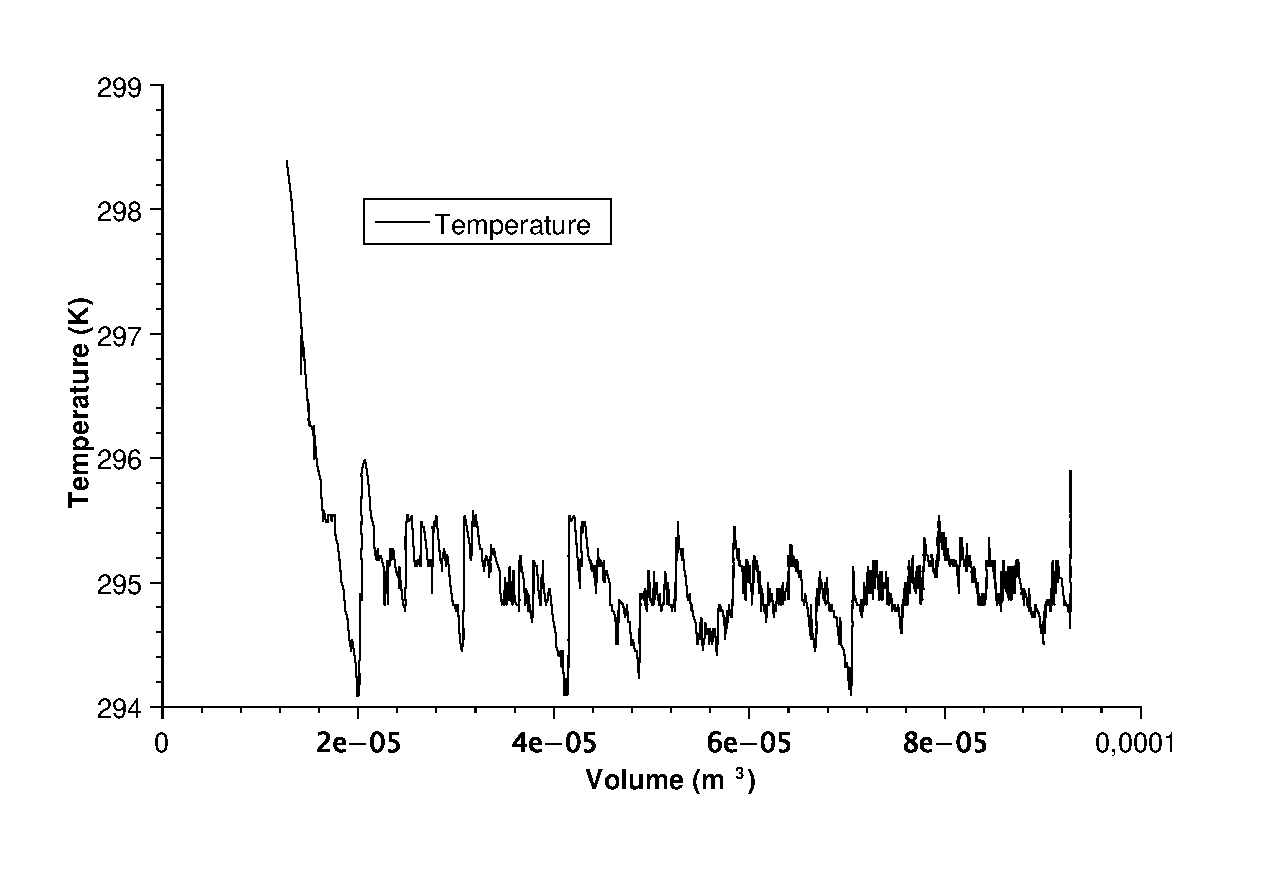
\includegraphics[width=0.5\textwidth]{3seg/TV_isothermal.eps}
    \caption{T(V) diagram for the isothermal process}
    \label{fig:TV_isothermal3}
\end{figure}
As one can see, it is not easy to hold a constant temperature experimentally, but it is visible on the graph that the temperature stays between 296 K and 294 K. If the Temperature would be perfectly constant, then we would get a straight line, meaning that the relation between temperature and volume in a isothermal process is a constant function.

For an adiabatic process, there is a relation between pressure and volume: \begin{equation} p V^{\gamma} = constant \label{eq:adiabaticConst}\end{equation} Whereas for an isothermal process there is the relation \begin{equation} T V^{\gamma - 1} = constant \label{eq:isothermalConst} \end{equation} In equation~(\ref{eq:adiabaticConst}) and equation~(\ref{eq:isothermalConst}) $\gamma$ is the so-called \textit{adiabatic index} \cite{adiabaticIndex}

%For an adiabatic process, the product of the pressure and volume stays constant. So, to verify the adiabatic process that goes from point 1 $\rightarrow$ point 2, we need to plot the pressure as a function of the inverse volume and determine the slope.
Since these relationships are valid at all times during the process, one can use two sets of data in equation~(\ref{eq:adiabaticConst}) to determine $\gamma$:
\begin{align*}
    p_1V_1^{\gamma} &= p_2V_2^{\gamma} \\
    \frac{V_1^{\gamma}}{V_2^{\gamma}} &= \frac{p_2}{p_1} \\
    ln \left[ \left( \frac{V_1}{V_2} \right)^{\gamma} \right] &= \ln\left(\frac{p_2}{p_1}\right)\\
    \gamma \ln\left(\frac{V_1}{V_2}\right) &= \ln\left(\frac{p_2}{p_1}\right)\\
\end{align*}

We are finally left with the relationship for $\gamma$ during an adiabatic process: \begin{equation}
    \gamma = \frac{\ln\left(\frac{p_2}{p_1}\right)}{\ln\left(\frac{V_1}{V_2}\right)}\\
\end{equation}   
    
When computing this value with the initial and end points, we get: $\gamma = 0.38$. We can then use this value to make a fit of our data in a $pV$ diagram, using $p = k \cdot V^{-\gamma}$: 

\begin{figure}[!ht]
    \centering
    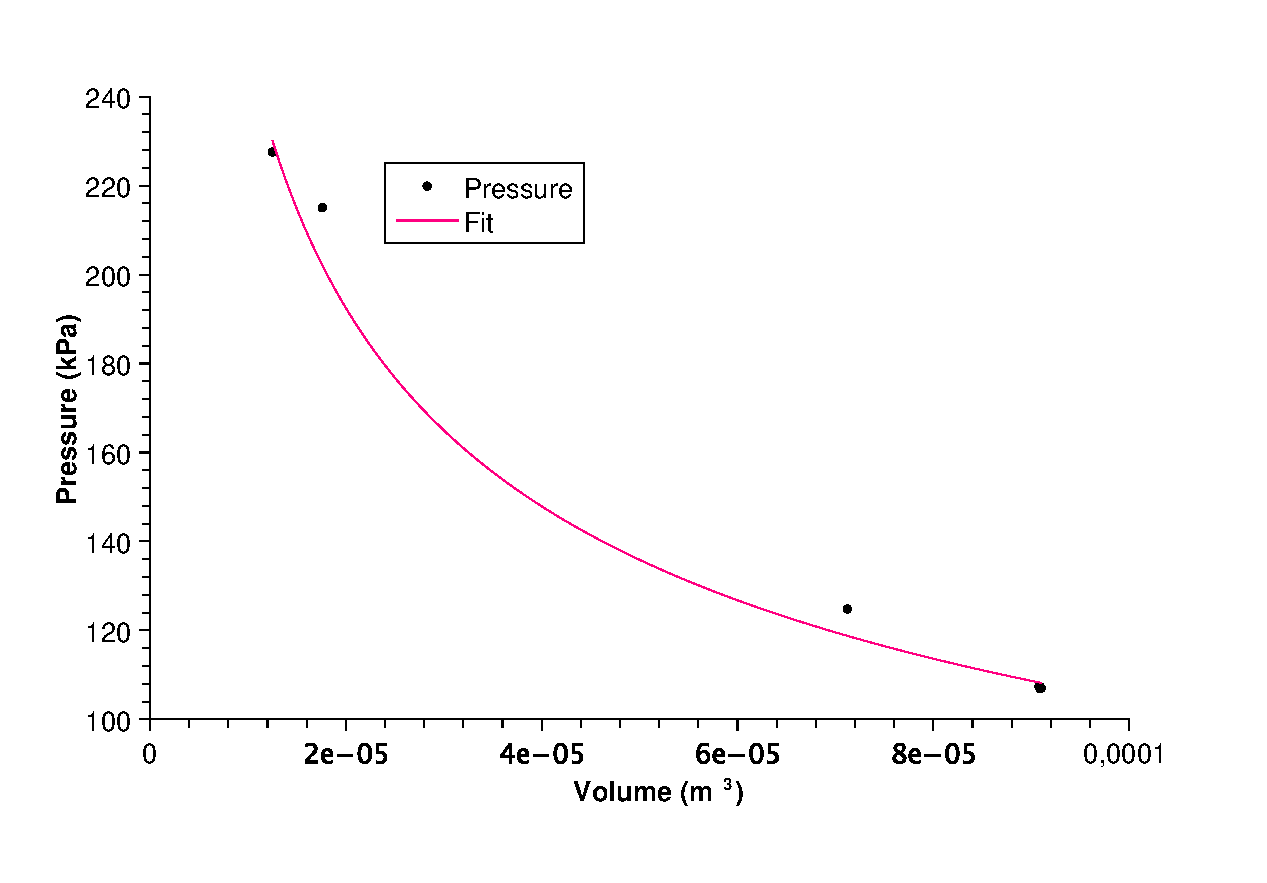
\includegraphics[width=0.5\textwidth]{3seg/adiabatic_3seg_gamma.eps}
    \caption{p(V) diagram for the adiabatic process}
    \label{fig:PV_adiabatic3}
\end{figure}
From this fit, we get the value of the constant, which is :
\[ \boxed{k = 3,15 \pm 0,06} \]

We can proceed in a similar fashion to determine $\gamma$ along the isothermal process using equation~(\ref{eq:isothermalConst}):
\begin{align*}
    T_1 V_1^{\gamma - 1} &= T_2 V_2^{\gamma - 1} \\
    \Leftrightarrow \quad \left( \frac{V_1}{V_2} \right)^{\gamma - 1} &= \frac{T_2}{T_1} \\
    \Leftrightarrow \quad (\gamma - 1 ) \ln{\left( \frac{V_1}{V_2} \right)} &= \ln \left( \frac{T_2}{T_1} \right) 
\end{align*}

%T3 und T1!!!!!

Which gives us again a formula for $\gamma$: 
\begin{equation}
    \gamma = \frac{ \ln \left( \frac{T_2}{T_1} \right)}{\ln{\left( \frac{V_1}{V_2} \right)}} + 1
\end{equation}

Finally, we can determine the change of internal energy and entropy.\vspace{0.3cm}

\textit{Adiabatic:}\\
The change of internal pressure is given by the following formula in the case of an adiabatic process:
\begin{equation}
    \Delta U_{12} = -\Delta W_{12}
\end{equation}
We get $W_{12}$ by integrating the PV diagram for the adiabatic section. This will be done on QTI-plot. We get an area of $-1.25 \cdot 10^{-2}$. So, the work from point 1 to point 2 is $W_{12} = -12.5$ J and thus:
\[\ \boxed{\Delta U_{12} = 12,5 \text{J} } \]\

Using the formula in table \ref{tab:formulas} we can also determine the specific heat for constant volume $C_V$
\begin{align*}
    \Delta U_{12} &= n_{air}C_V\Delta T\\
    C_V &= \frac{\Delta U_{12}}{n_{air}(T_2-T_1)}\\
    &= \boxed{68.5 \ \text{J} \cdot \text{mol}^{-1} \cdot \text{K}^{-1}}
\end{align*}
The change of entropy for an adiabatic process is 0.\vspace{0.3cm}

\textit{Isochoric:}\\
The change of internal energy for the isochoric process is:
    \begin{align*}
        \Delta U_{23} &= nC_V\Delta T\\
        &= 2.83 \cdot 10^{-3} \cdot 68.5\cdot (298.39-362.85)\\
        &= \boxed{-12.45 \ \text{J} \cdot \text{mol}^{-1} \cdot \text{K}^{-1}}
    \end{align*}
The change of entropy is:
    \begin{align*}
        \Delta S_{23} &= nC_V \ln\left(\frac{T_3}{T_2}\right)\\
        &= 2.83 \cdot 10^{-3} \cdot 68.5\cdot \ln\left(\frac{298.39}{362.85}\right)\\
        &= \boxed{-0.038 \ \text{J} \cdot \text{K}^{-1}}
    \end{align*}
\vspace{0.3cm}

\textit{Isothermal:}\\
The change of internal energy for an isothermal process is 0.\\
The change of entropy is:
    \begin{align*}
        \Delta S_{31} &= nR\ln\left(\frac{V_1}{V_3}\right)\\
        &= 2.83 \cdot 10^{-3} \cdot 8.314\cdot \ln\left(\frac{9.09 \cdot 10^{-5}}{1.27 \cdot 10^{-5}}\right)\\
        &= \boxed{0.046 \ \text{J} \cdot \text{K}^{-1}}
    \end{align*}
\vspace{0.3cm}

\textit{Total change in internal energy}
\[ \Delta U_{total} = 0.05 \ \text{J} \]

\textit{Total change in entropy}
\[ \Delta S_{total} = 0.008  \ \text{J} \cdot \text{K}^{-1} \]

We can observe that there is a slight increase in internal energy in the system. The internal energy we put  in during the adiabatic process, is also put out, with nearly the same value, during the isochoric one.\\
Additional, we have also a small increase in entropy. The change of entropy during the isothermal process is much larger than during the isochoric process. We can also add, that for the isochoric process, the change in entropy shoulnd't be negative.
\subsubsection{P(V) diagrams of other gases}
\begin{figure}[!ht]
     \centering
     \begin{subfigure}[b]{0.3\textwidth}
         \centering
         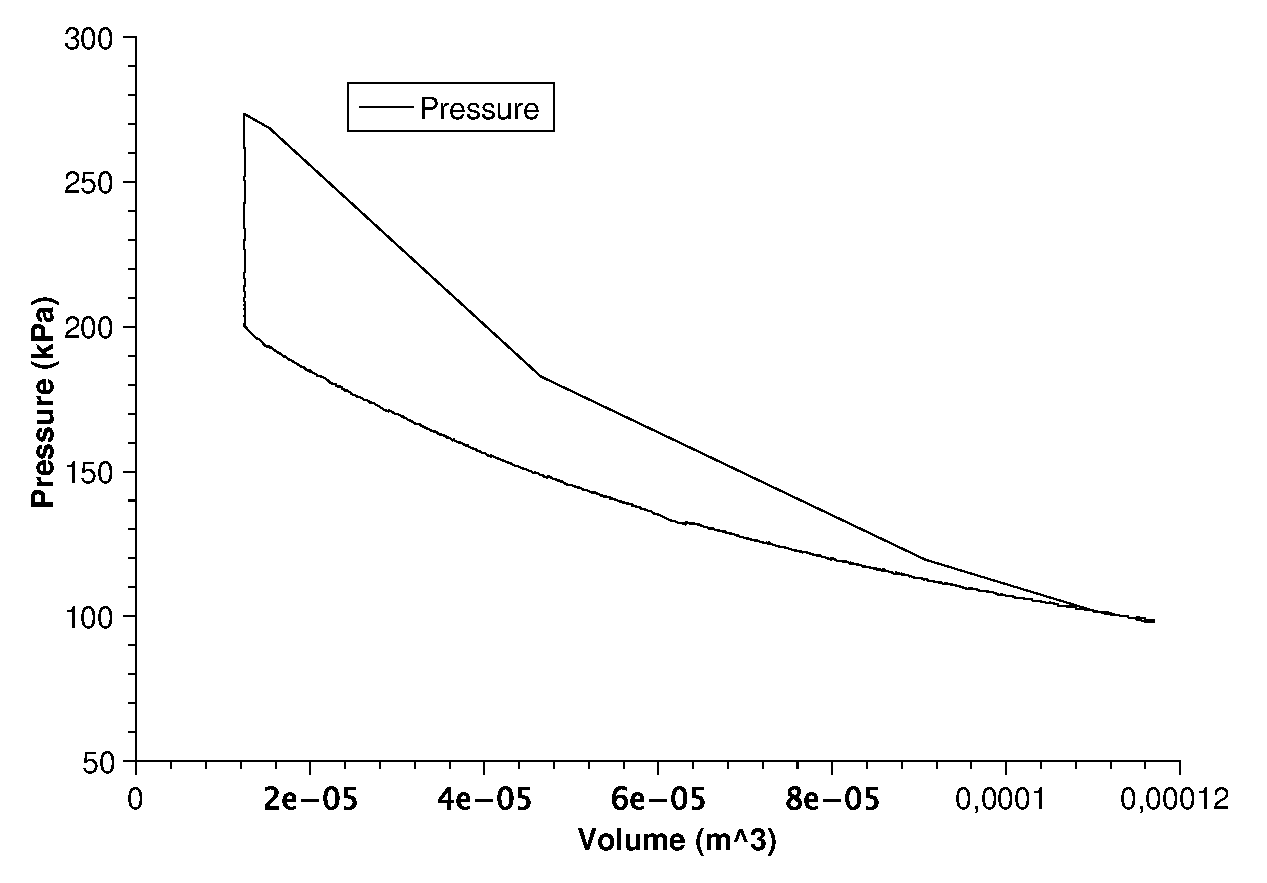
\includegraphics[width=\textwidth]{3seg/PV_argon_3.eps}
         \caption{Three-segment cycle P(V) diagram for argon}
         \label{fig:3seg_argon}
     \end{subfigure}
     \hfill
     \begin{subfigure}[b]{0.3\textwidth}
         \centering
         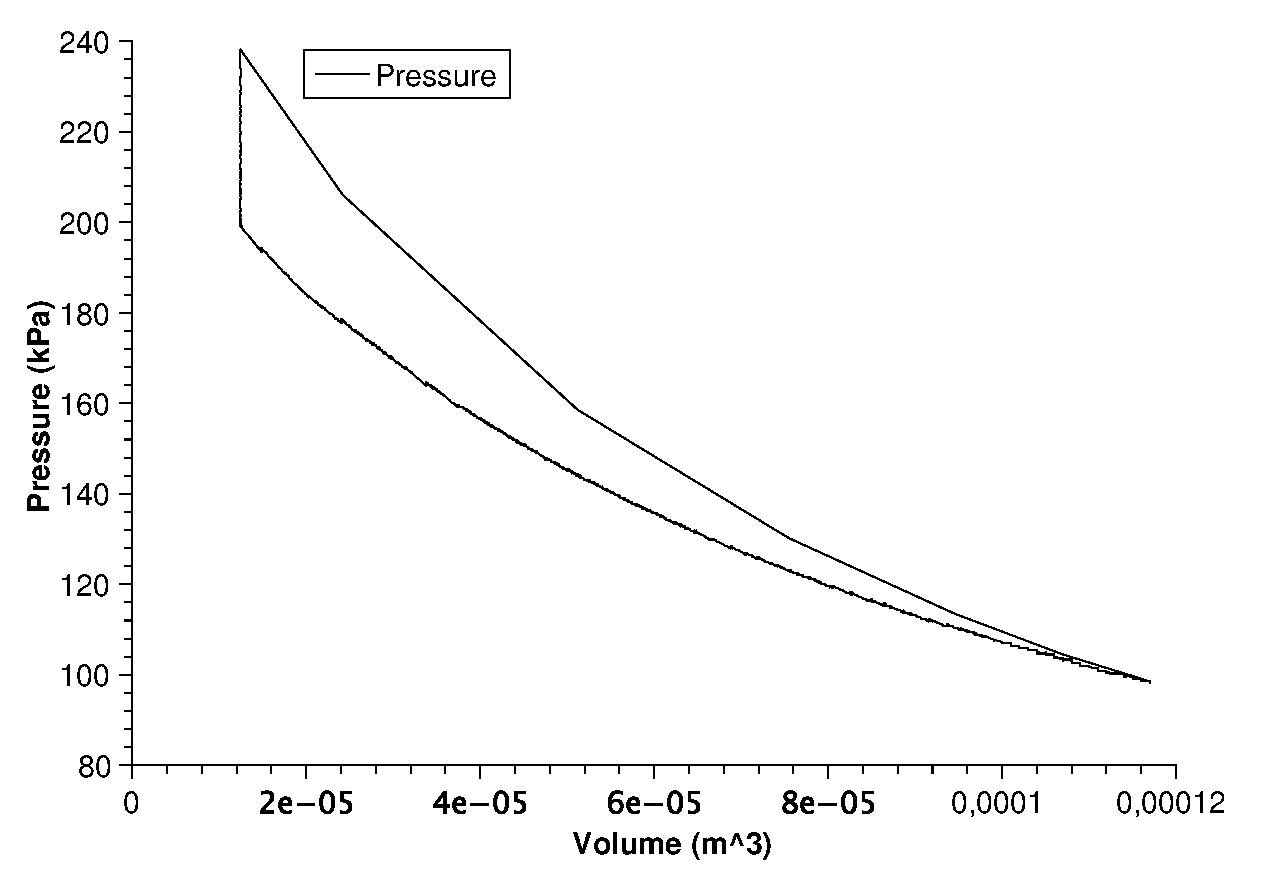
\includegraphics[width=\textwidth]{3seg/PV_CO2_3seg.eps}
         \caption{Three-segment cycle P(V) diagram for Carbon dioxide}
         \label{fig:3seg_CO2}
     \end{subfigure}
     \hfill
     \begin{subfigure}[b]{0.3\textwidth}
         \centering
         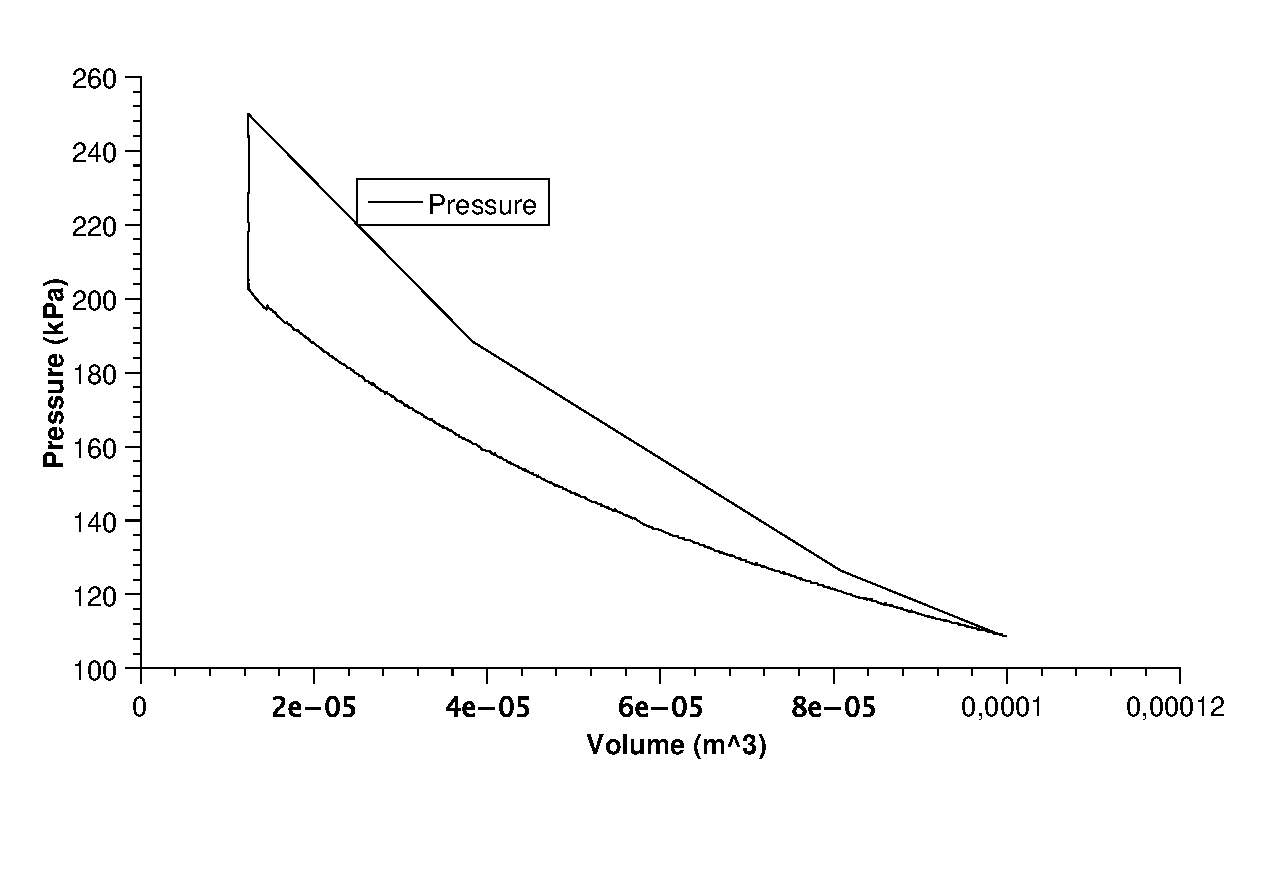
\includegraphics[width=\textwidth]{3seg/PV_helium_3seg.eps}
         \caption{Three-segment cycle P(V) diagram of helium}
         \label{fig:3seg_helium}
     \end{subfigure}
\end{figure}
\FloatBarrier


\subsection{Reversed Otto cycle}

\subsubsection{Air}
Figure~(\ref{fig:pVOttoAir}) shows the resulting P(V) diagram of the reversed Otto cycle of air.
\begin{figure}[!ht]
    \centering
    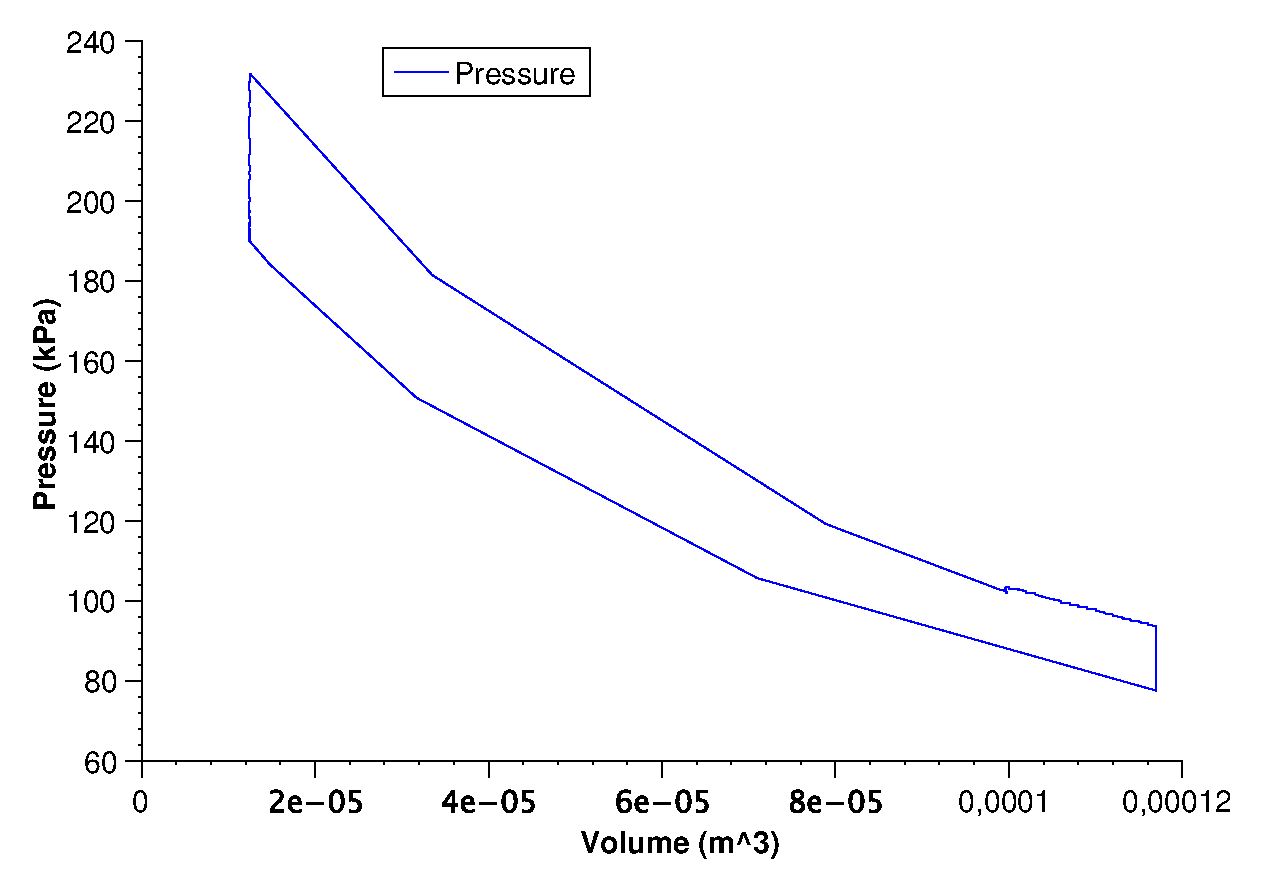
\includegraphics[width=0.5\textwidth]{PV_air_O.eps}
    \caption{P(V) diagram for the reversed Otto cycle of air}
    \label{fig:pVOttoAir}
\end{figure}

The limiting points for the reversed Otto cycle (see figure \ref{fig:Otto pic}) corresponding to the above P(V) diagram  are:

\begin{table}[!ht]
    \centering
    \begin{tabular}{c|c|c|c}
        point & V ($m^3$) & p (kPa) & T (K)  \\
        \hline
        1 & $9,97 \cdot 10^{-5}$ & 102,42 & 296,99\\
        2 & $1,25 \cdot 10^{-5}$ & 231,93 & 366,1\\
        3 & $1,25 \cdot 10^{-5}$ & 189,97 & 298,8 \\
        4 & $1,17 \cdot 10^{-4}$ & 77,64 & 256,46
    \end{tabular}
    \caption{Data points the reversed Otto cycle of air}
    \label{tab:Data_airOtto}
\end{table}

\textbf{Variation of internal energy and entropy}

\textit{Adiabatic compression:}
\begin{align*}
    \Delta U_{12} &= nc_V \Delta T \\
    &= nc_V(T_2 - T_1) \\
    &= 2.83 \cdot 10^{-3} \ \text{mol} \cdot 68.5 \ \text{J} \cdot \text{mol}^{-1} \cdot \text{K}^{-1} \cdot (366.1-296.81) \ \text{K} \\
    &= 13.43 \ \text{J} \\
    \Delta S_{12} &= 0
\end{align*}

\textit{Isochoric cooling}
\begin{align*}
    \Delta U_{23} &= nc_V \Delta T \\
    &= nc_V(T_3 - T_2) \\
    &= 2.83 \cdot 10^{-3} \ \text{mol} \cdot 68.5 \ \text{J} \cdot \text{mol}^{-1} \cdot \text{K}^{-1} \cdot (372.12 - 298.8) \ \text{K} \\
    &= -14.21 \ \text{J} \\
    \Delta S_{23} &= nc_V \ln \left( \frac{T_3}{T_2} \right) \\
    &= 2.83 \cdot 10^{-3} \ \text{mol} \cdot 68.5 \ \text{J} \cdot \text{mol}^{-1} \cdot \text{K}^{-1} \cdot \ln \left( \frac{372.12}{298.8} \right) \\
    &= 0.043 \ \text{J} \cdot \text{K}^{-1}
\end{align*}

\textit{Adiabatic expansion}
\begin{align*}
    \Delta U_{34} &= nc_V \Delta T \\
    &= nc_V(T_4 - T_3) \\
    &= 2.83 \cdot 10^{-3} \ \text{mol} \cdot 68.5 \ \text{J} \cdot \text{mol}^{-1} \cdot \text{K}^{-1} \cdot (256.46-298.8) \ \text{K} \\
    &= -8.21 \ \text{J} \\
    \Delta S_{34} &= 0
\end{align*}

\textit{Isochoric heating}
\begin{align*}
    \Delta U_{41} &= nc_V \Delta T \\
    &= nc_V(T_1 - T_4) \\
    &= 2.83 \cdot 10^{-3} \ \text{mol} \cdot 68.5 \ \text{J} \cdot \text{mol}^{-1} \cdot \text{K}^{-1} \cdot (300.47-256.46) \ \text{K} \\
    &= 8.53 \ \text{J} \\
    \Delta S_{41} &= nc_V \ln \left( \frac{T_1}{T_4} \right) \\
    &= 2.83 \cdot 10^{-3} \ \text{mol} \cdot 68.5 \ \text{J} \cdot \text{mol}^{-1} \cdot \text{K}^{-1} \cdot \ln \left( \frac{300.47}{256.46} \right) \\
    &= 0.031 \ \text{J} \cdot \text{K}^{-1}
\end{align*}

\textit{Total change in internal energy}
\begin{equation*}
    \Delta U_{total} = -0.46 \ \text{J}    
\end{equation*}
\textit{Total change in entropy}
\begin{equation*}
    \Delta S_{total} = 0.073 \ \text{J} \cdot \text{K}^{-1}   
\end{equation*}

We can see that the system lost internal energy, despite us doing work on the system externally. The change in internal energy is bigger during the adiabatic compression than during the adiabatic expansion, which occurs at lower temperatures. A significant amount of internal energy was lost during the isochoric cooling, as the air temperature was reduced by about $70$ K, whereas during the isochoric heating its temperature was only raised by about $40$ K. The loss of internal energy during the isochoric cooling is also bigger than the gain through adiabatic compression.

Furthermore, the entropy is increasing during the cycle, respecting the law $\Delta S > 0$. The gain in entropy is actually greater during the isochoric cooling than during the isochoric heating process. In theory, the entropy does not increase during adiabatic processes, however these are hard to realize perfectly in reality. We therefore considered the change in entropy during the adiabatic expansion and adiabatic compression to be 0, but there has very certainly been a - minimal - increase in entropy. This increase is however much smaller than the change due to the isochoric processes and can therefore be disregarded.

\subsubsection{P(V) diagram for other gases}
\begin{figure}[!ht]
     \centering
     \begin{subfigure}[b]{0.3\textwidth}
         \centering
         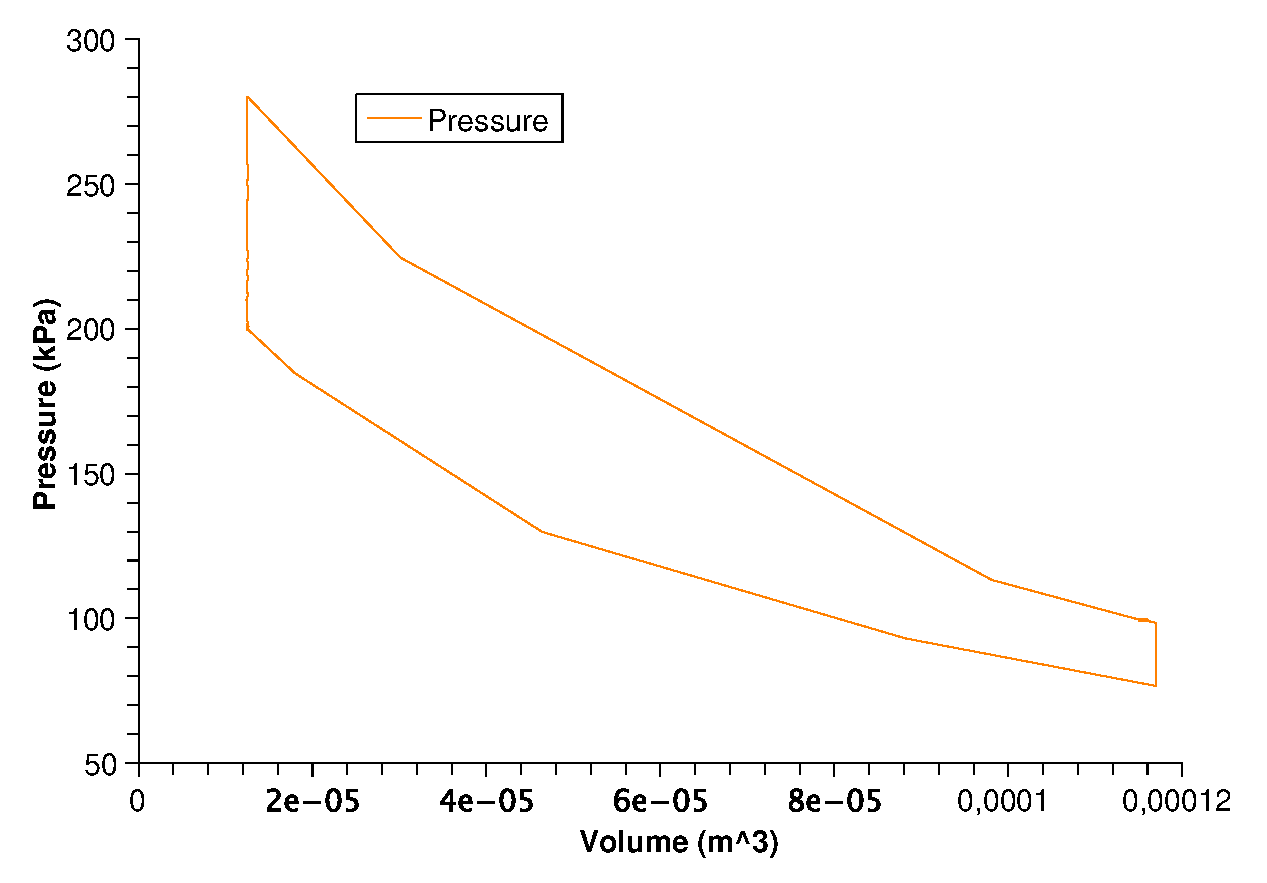
\includegraphics[width=\textwidth]{Otto/PV_argon_O.eps}
         \caption{Reversed Otto cycle P(V) diagram for argon}
         \label{fig:Otto_argon}
     \end{subfigure}
     \hfill
     \begin{subfigure}[b]{0.3\textwidth}
         \centering
         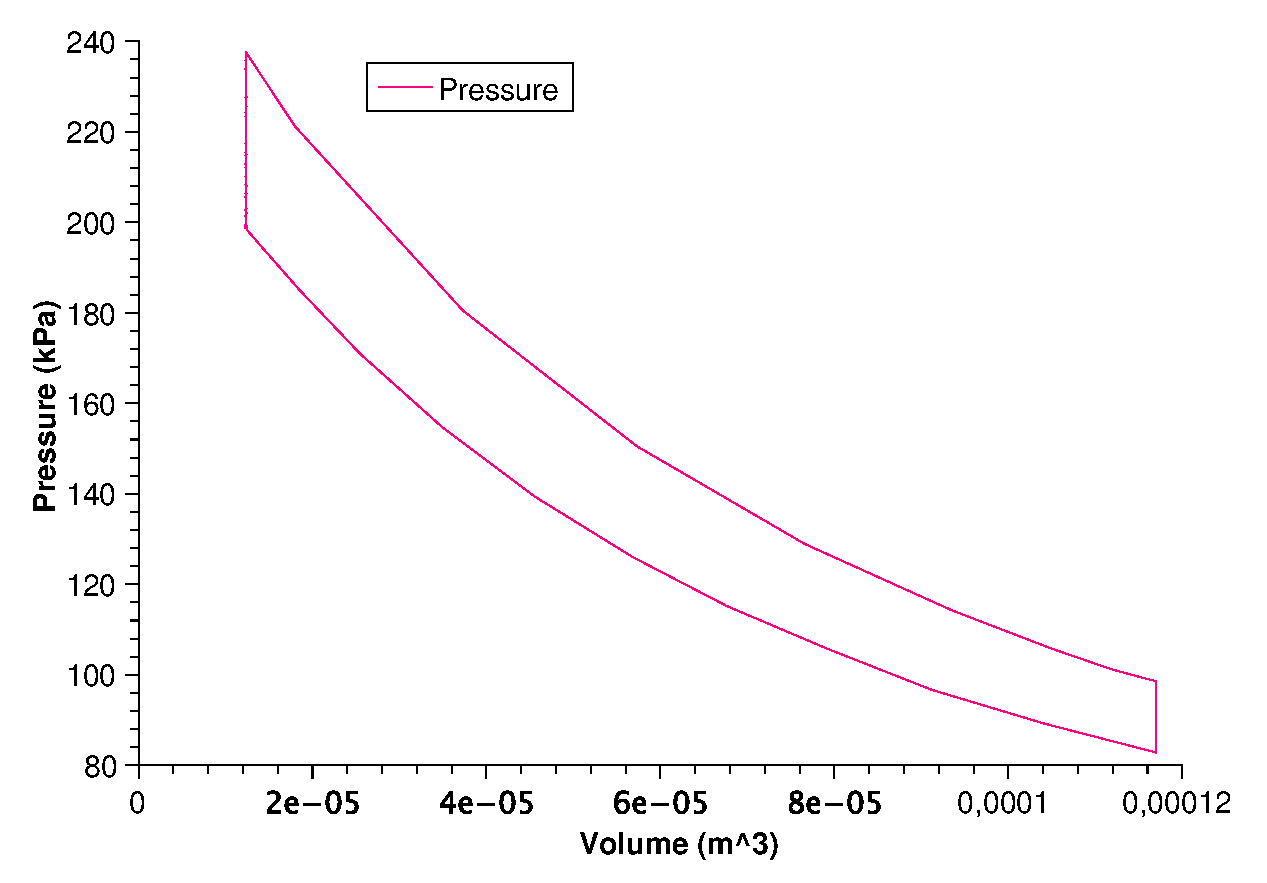
\includegraphics[width=\textwidth]{Otto/PV_CO2_Otto.eps}
         \caption{Reversed Otto cycle P(V) diagram for Carbon dioxide}
         \label{fig:Otto_CO2}
     \end{subfigure}
     \hfill
     \begin{subfigure}[b]{0.3\textwidth}
         \centering
         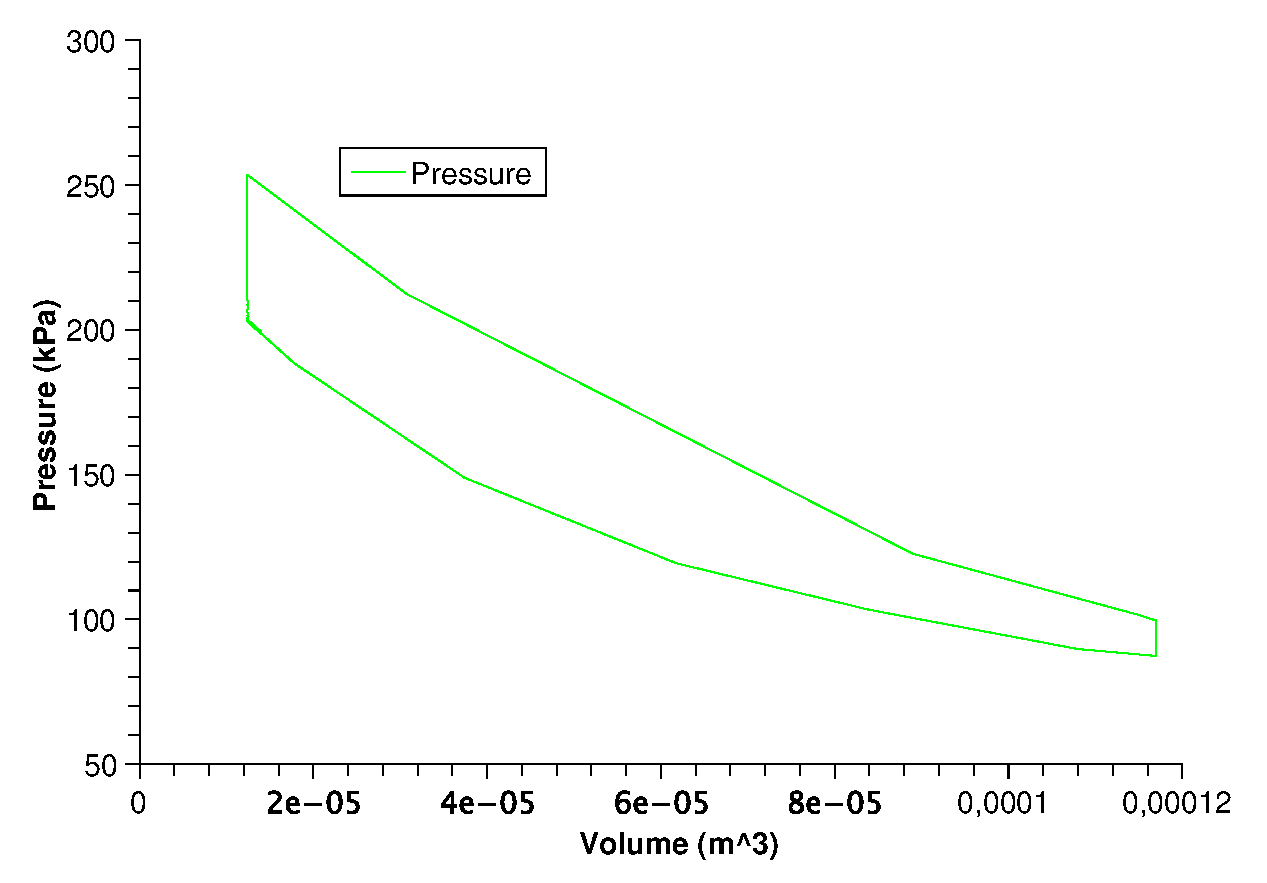
\includegraphics[width=\textwidth]{Otto/PV_helium_Otto.eps}
         \caption{Reversed Otto cycle P(V) diagram of helium}
         \label{fig:Otto_helium}
     \end{subfigure}
\end{figure}
\FloatBarrier


\section{Conclusion}

Through the study of the three-segment cycle and the reversed Otto cycle, we were able to determine the heat capacity of air: $c_V = 68.5 \ \text{J} \cdot \text{mol}^{-1} \cdot \text{K}^{-1}$, and study the adiabatic, isothermal and isochoric processes with our heat engine. We have found that we can modify the internal energy of the system via compression and cooling, or expansion and heating of the gas inside. The change in internal energy and entropy was also noticeable. 
For the three-segment cycle of air, the change in internal energy $\Delta U_{total}$ is 0.05 J and the change of entropy $\Delta S_{total} = 0.008 \ J\cdot K^{-1}$. On the other hand for the reversed Otto cycle of air, $\Delta U_{total} = -0.46 \ J$ and $\Delta S_{total} = 0.0073 \ J\cdot K^{-1}$.
Despite the closed system, a loss of internal energy can be seen for the reversed Otto cycle. One reason for this could be that the valves are never tightly closed and therefore some gas escapes during manipulation.\\


\begin{thebibliography}{}
    \bibitem{} Lab guide, Jörg Baller, version 1.2, March 2021
    \bibitem{adiabaticIndex} \textit{Adiabatic process}, Wikipedia,  \url{https://en.wikipedia.org/wiki/Adiabatic_process}, accessed 19/04/22
    \bibitem{isochoricProcess} \textit{Isochoric process}, Wikipedia, \url{https://en.wikipedia.org/wiki/Isochoric_process}, accessed 21/04/22
    \bibitem{isothermalProcess} \textit{Isothermal process}, Wikipedia, \url{https://en.wikipedia.org/wiki/Isothermal_process}, accessed 21/04/22
\end{thebibliography}

\end{document}
